% 基于互联网的创意设计
% LaTeX Template
% Version 1.0 
\documentclass{ctexart} % 默认为5号(pt=10.5)字体,pt越大字体越大
\linespread{1.2} % 行距为1.2
\usepackage{url}  % 使用宏包url提供超链接
\usepackage{graphicx}
\usepackage[top=1.5cm, bottom=3cm, left=2.5cm, right=2.5cm]{geometry}  % 使用geometry来控制页面布局
\title{\centering {\LARGE{基于互联网的创意设计}\\ \small{——扎克伯格的Jarvis}}\\% Title
} % Subtitle
\author{\textsc \small{{陈李锋 14通信 2014081025 }} % Author
} % Institution

%----------------------------------------------------------------------------------------

\begin{document}

\maketitle % Print the title section

\begin{abstract} %摘要
Facebook的CEO扎克伯格(Mark Zuckerbarg)在他的2016年年度计划中定的目标为做一个AI管家Jarvis(钢铁侠里面那个智能管家)。
在2016年的12.20 日,扎克伯格在 Facebook 的blog 上发布文章,说自己已经搞定了,一共用了大概 100 个小时(大部分都是现有的技术),
同时他也表达了自己对人工智能的一些看法。

本文首先介绍了扎克伯格的Jarvis,然后对比同类产品Google Home和Amazon Echo等中央控制系统,最后总结是中控与人工智能关系。
\\关键词: Jarvis\quad  Google Home \quad Amazon Echo \quad 人工智能 

\end{abstract}

\subsubsection*{\raggedleft{扎克伯格的Jarvis}}
\paragraph{}
自从 2009 年至今,扎克伯格每年都会制定一个新年目标,比如之前的「每天戴领带上班」、「每天写一封感谢信」、「学汉语」、「每天写代码」等,而 2015 年年末,他定的目标是做一个 AI 管家 Jarvis。

AI 管家 Jarvis使用文字和语音来交互,做的事情虽然不是很难,比如开关灯,打开放家里的家用电器,根据口味推荐菜单,家庭安全如让熟人进门,控制汽车开关门之类的。为了实现Jarvis,扎克伯格Python,php,和 OC 编写 Jarvis。下图是项目架构。

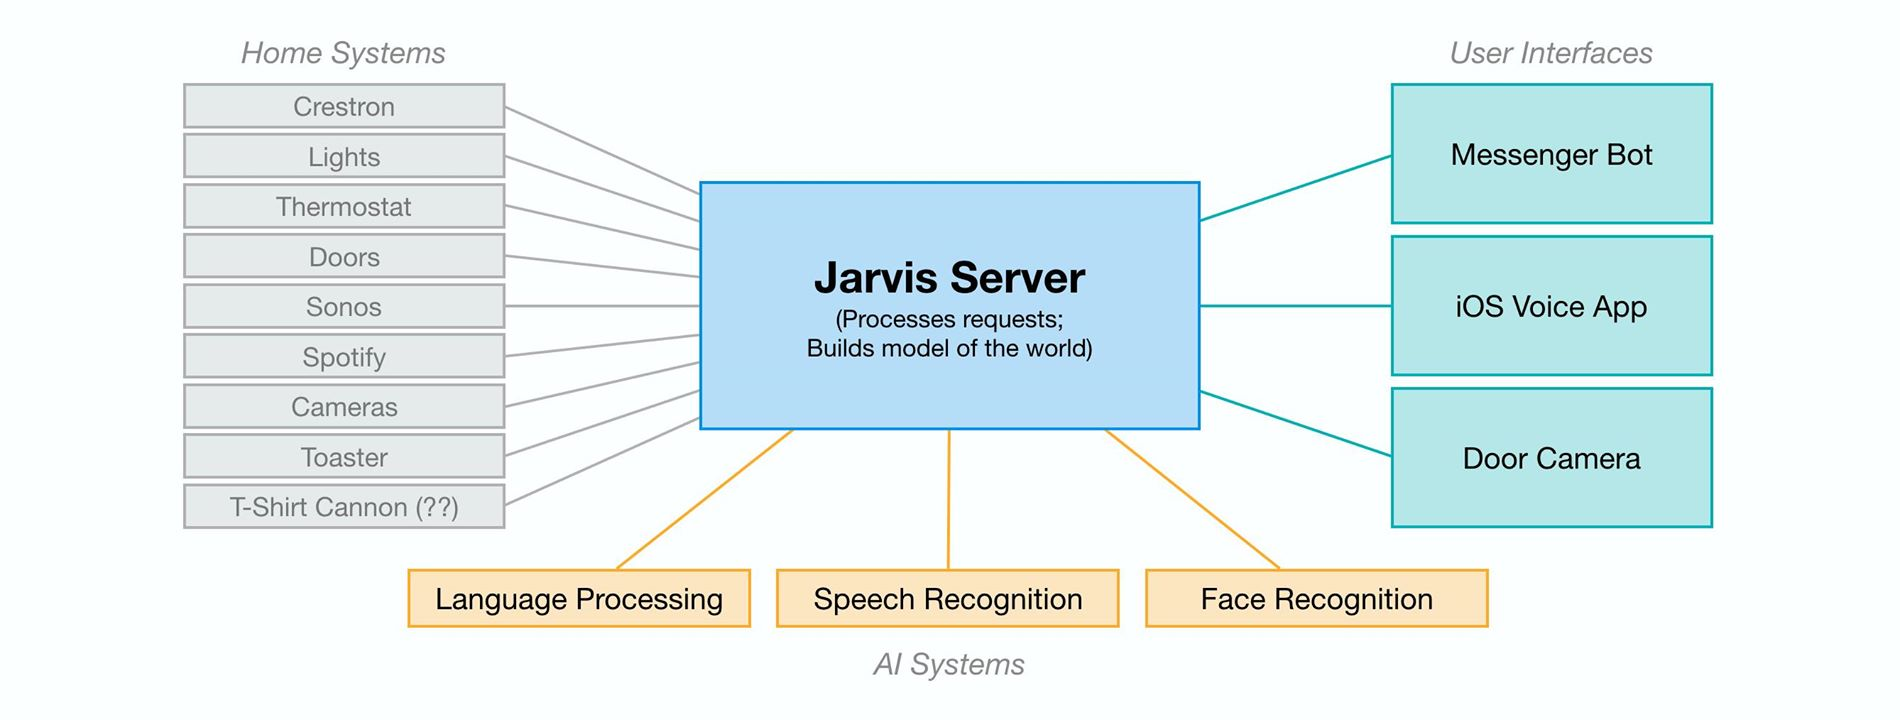
\includegraphics[width=1.0\linewidth]{Jarvis_structer}
主要步骤为:

第一步,扎克伯格他先让 Jarvis 和家用电器通过互联网连接。不论是面包机还是衣柜,都要智能的连接才能够融入 Jarvis 系统。

第二步,自然语言。最开始扎克伯格是采用文本方式来控制,后来增加了语音控制功能。Jarvis 通过关键字如「床」、「灯」、「食物」等来判断,通过反复自我学习来训练理解上下文。

第三步,视觉训练和面部识别。他赋予 Jarvis 动态视觉跟踪能力,比如孩子醒了,或者家里有什么风吹草动,都会得到反馈。另外结合了Facebook 的强大面部识别功能,当朋友站在门口,就能识别出这是谁,Jarvis 判断后可以给这个人开门。他说视觉能力在 Jarvis 上非常重要,也有更多能开发的有意思的功能。

第四步,信息反馈。Jarvis 能根据主人的语句来给于反馈(Siri、微软小冰都能做到)。

第五步,语音和识别。给 Jarvis 添加声音。
\subsubsection*{\raggedleft{对比同类产品}}
\paragraph{}
 简单讲,扎克伯格搞了个智能家居领域的中央控制系统(中控)。中控作为中间层,一端是人输入的基于关键字的简单指令,而另一端是第三方软件应用。而Jarvis AI一端是人输入的自然指令,另一端是家居设备。最为核心的人工智能模块,就是用于把人输入的自然指令,转化成为机器指令。
 
 Amazon的echo,Google 的google home ,还有国内的rokid的 pebble 这三个人工智能产品在本质上和Jarvis是一样的,都是市场上售卖或者预售的中控。它们表面上来看是一个语音智能音箱,但实质上是一个面向未来的产品,也将会成为一种新的流量入口。它有别于传统的PC和手机交互方式,是全新的基于自然语言的交互方式,更自然,更简单,也更聪明。

\subsubsection*{\raggedleft{中控与人工智能关系}}
\paragraph{}
扎克伯格所做的Jarvis AI 很好地展示了人工智能技术目前所处的阶段:人工智能领域到目前为止的成果已经远超大多数人的预料,但与此同时,我们离电影中那种「真正的智能」还很远。同时他也对当前AI领域的判断:AI离我们既近又远。它已经能做很多有意义的事,其中的某些很快就会比人类自己做得更好。但与此同时,我们还在摸索真正的智能是什么。

智能家居的发展难题现在除了在探索发展方向之外,另外一个是没有统一的系统和标准,各自为战。虽然强大足够智能的AI无法短时间内实现,但制定统一的系统和标准,同样可以大幅提高智能家居的实用性,使之进入千家万户,而不是一个鸡肋般的功能。但让人遗憾的是,目前智能家居的现状是,接口不统一,协议不公开。且厂商之间互相竞争,虽然出现了大量的智能家具,但从没考虑过兼容的事情。
但罗马不是一天就能建起来,凡事都有过程,相信随着更多企业涌入智能设备领域,产品也会快速迭代,相信用不了多久,智能家居就能取得不错的突破,进入到我们的生活。

\subsubsection*{结语}
  Jarvis的实现,是扎克伯格基于钢铁侠的一个创意产品。他也是想通过这个,了解到了目前人类在AI方面的技术发展程度。AI的发展非常迅速,年初的阿法狗战胜李世石事件,让人类第一次感受到了AI某种程度上的强大。扎克伯格表示,AI系统将拥有比人类更加准确的视觉、听觉、触觉等等。但现在的人工智能,只是较低水平的只能,因为类似Jaivis的还没有完全的自主学习能力。毕竟,距离真正的强大的人工智能,我们还有太远的距离要走。
\\ \\ \\ 参考文献:

[1] Mark-Zuckerberg.Building-Jarvis. \url{ //www.facebook.com/notes/mark-zuckerberg/building-jarvis} 

[2] 外媒Theverge对Jarvis的报道.

 \url{https://www.theverge.com/mark-zuckerberg-jarvis-home-ai-video-watch}

[3] Echo,Home和Rokid的比较.关伟强. \url{https://www.zhihu.com/question/59071372/answer/165159990}


\end{document}
